\documentclass{article}

% Language setting
% Replace `english' with e.g. `spanish' to change the document language
\usepackage[english]{babel}

% Set page size and margins
% Replace `letterpaper' with`a4paper' for UK/EU standard size
\usepackage[letterpaper,top=2cm,bottom=2cm,left=3cm,right=3cm,marginparwidth=1.75cm]{geometry}

% Useful packages
\usepackage{amsmath}
\usepackage{graphicx}
\usepackage{subcaption}
\usepackage{float}
\usepackage[outputdir=build]{minted}
\usepackage[colorlinks=true, allcolors=blue]{hyperref}
\usepackage{amssymb}
\usepackage{tcolorbox}

\title{DeepLearning.ai - LangChain Chat with Your Data}
\author{Elena Figueira Rodríguez}

\begin{document}
\maketitle

\begin{abstract}

\end{abstract}

\maketitle

% Table of Contents
\tableofcontents

\newpage  % Start the content on a new page

%%%%%%%%%%%%%%%%%%%% SECTION %%%%%%%%%%%%%%%%%%%%
\section{Introduction}

Hi, I'm excited to share with you this new course on using LangChain to chat with your data. This is built in collaboration with Harrison Chase, co-founder and CEO of LangChain.

%%%%%%%%%%%%%%%%% SUBSECTION %%%%%%%%%%%%%%%%%
\subsection{Understanding Large Language Models}

Large language models (LLMs) such as ChatGPT can answer questions about a lot of topics, but an LLM in isolation knows only what it was trained on. This means it does not include your personal data. 

For example, if you're in a company and have proprietary documents that are not available on the internet, or if you need access to data or articles written after the LLM was trained, it would not have access to that information.

Wouldn't it be useful if you or others, such as your customers, could have a conversation with your own documents and get questions answered using information from those documents while leveraging an LLM?

%%%%%%%%%%%%%%%%% SUBSECTION %%%%%%%%%%%%%%%%%
\subsection{Using LangChain for Data Interaction}

LangChain is an open-source developer framework for building LLM applications. It consists of several modular components as well as more end-to-end templates.

%%%%%%%%%%%%%% SUBSUBSECTION %%%%%%%%%%%%%%
\subsubsection{Core Components of LangChain}

The modular components in LangChain include:

\begin{itemize}
    \item Prompts
    \item Models
    \item Indexes
    \item Chains
    \item Agents
\end{itemize}

\begin{figure}[H]
    \centering
    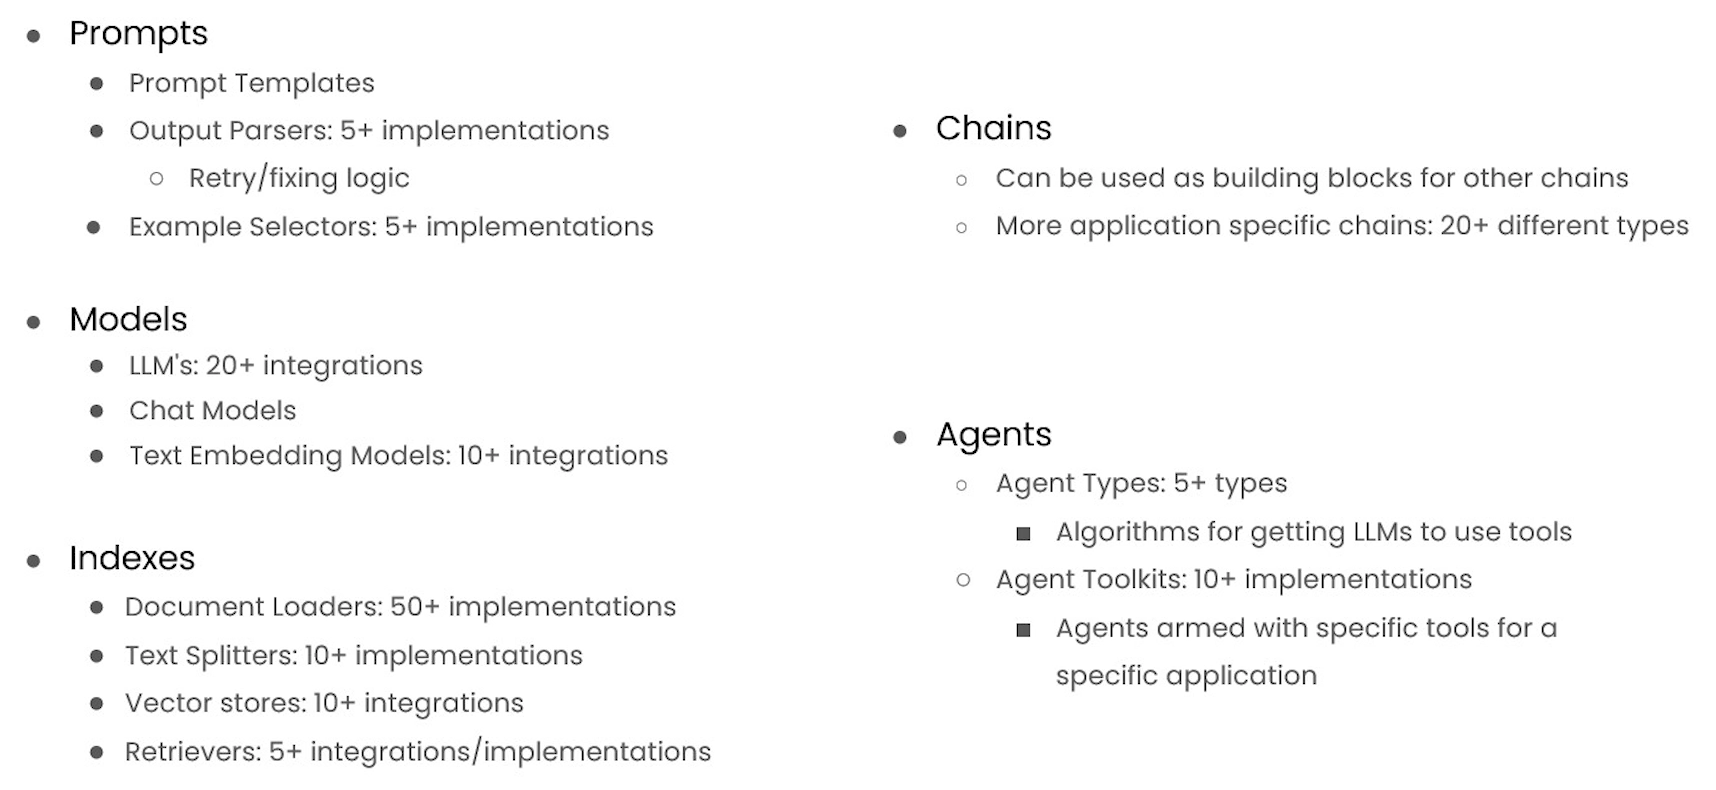
\includegraphics[width=0.8\textwidth]{images/langchain_chat_with_your_data_001.png}
    \caption{Introduction - Core Components of LangChain}
    \label{fig:introduction_core_components_of_langchain}
\end{figure}

For a more detailed look at these components, you can refer to our first course that I taught with Andrew.

%%%%%%%%%%%%%% SUBSUBSECTION %%%%%%%%%%%%%%
\subsubsection{A Focus on Chatting with Data}

In this course, we will zoom in and focus on one of the more popular use cases of LangChain—\textbf{how to use LangChain to chat with your data}. We will first cover \textbf{how to use LangChain document loaders} to load data from a variety of exciting sources.

\begin{figure}[H]
    \centering
    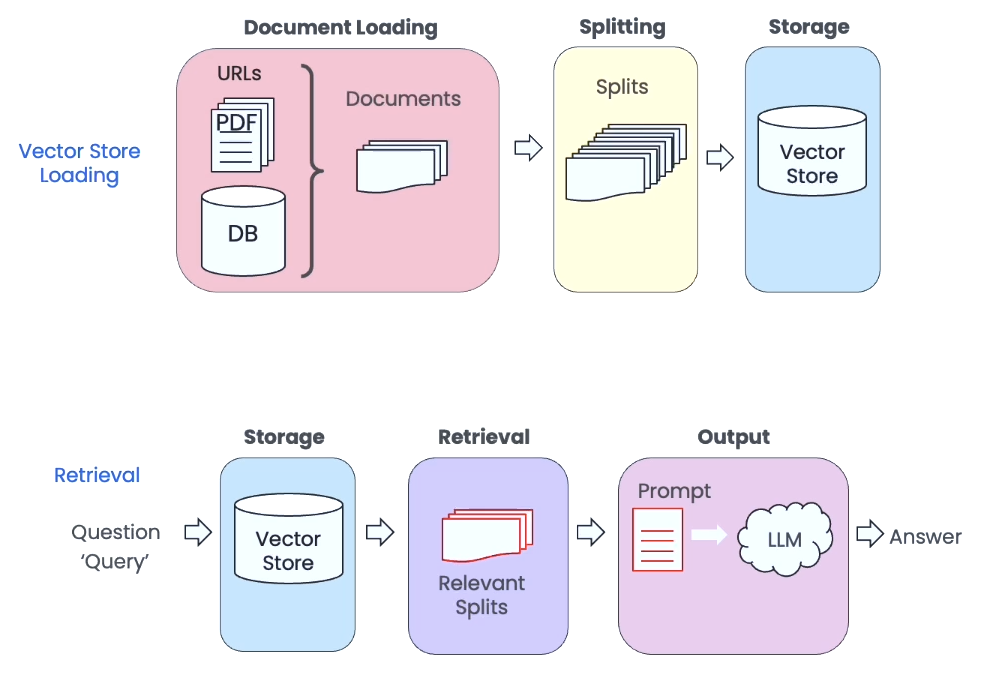
\includegraphics[width=0.8\textwidth]{images/langchain_chat_with_your_data_002.png}
    \caption{Introduction - RAG Schema}
    \label{fig:introduction_rag_schema}
\end{figure}

We will then touch on how to split these documents into semantically meaningful chunks. This pre-processing step may seem simple but has a lot of nuances.

Next, we will give an \textbf{overview of semantic search}, a basic method for fetching relevant information given a user question. This is the easiest method to get started with, but there are several cases where it fails. We'll go over these cases and then explore how to fix them.

We'll then show \textbf{how to use those retrieved documents to enable an LLM to answer questions about a document}. However, we’ll also highlight that you're still missing one key piece in order to fully recreate that chatbot experience.

Finally, we'll cover that missing piece—\textbf{memory}—and show \textbf{how to build a fully functioning chatbot through which you can chat with your data}.

%%%%%%%%%%%%%%%%% SUBSECTION %%%%%%%%%%%%%%%%%
\subsection{Conclusion}
With that, let us now move on to the next video where Harrison will show you how to use LangChain's very convenient collection of document loaders.

%%%%%%%%%%%%%%%%%%%% SECTION %%%%%%%%%%%%%%%%%%%%
\section{Document Loading}

%%%%%%%%%%%%%%%%% SUBSECTION %%%%%%%%%%%%%%%%%
\subsection{Introduction}
In order to create an application where you can chat with your data, you first have to load your data into a format where it can be worked with. That's where LangChain document loaders come into play. 

LangChain provides over 80 different types of document loaders. In this lesson, we'll cover a few of the most important ones and help you get comfortable with the concept in general.

%%%%%%%%%%%%%%%%% SUBSECTION %%%%%%%%%%%%%%%%%
\subsection{Understanding Document Loaders}

Document loaders deal with the specifics of accessing and converting data from a variety of different formats and sources into a standardized format. 

There are different places from which we may want to load data, including:

\begin{itemize}
    \item Websites
    \item Various databases
    \item YouTube videos
    \item arXiv
    \item ...
\end{itemize}

Additionally, documents can come in different data types, such as:

\begin{itemize}
    \item PDFs
    \item HTML
    \item JSON
    \item Word, PowerPoint
    \item ...
\end{itemize}

The main role of document loaders is to take this variety of data sources and load them into a standard document object, which consists of:

\begin{itemize}
    \item Content
    \item Associated metadata
\end{itemize}

%%%%%%%%%%%%%%%%% SUBSECTION %%%%%%%%%%%%%%%%%
\subsection{Types of Document Loaders}
There are many different types of document loaders in LangChain. While we won’t cover all of them, we can broadly categorize them into these groups:

\begin{figure}[H]
    \centering
    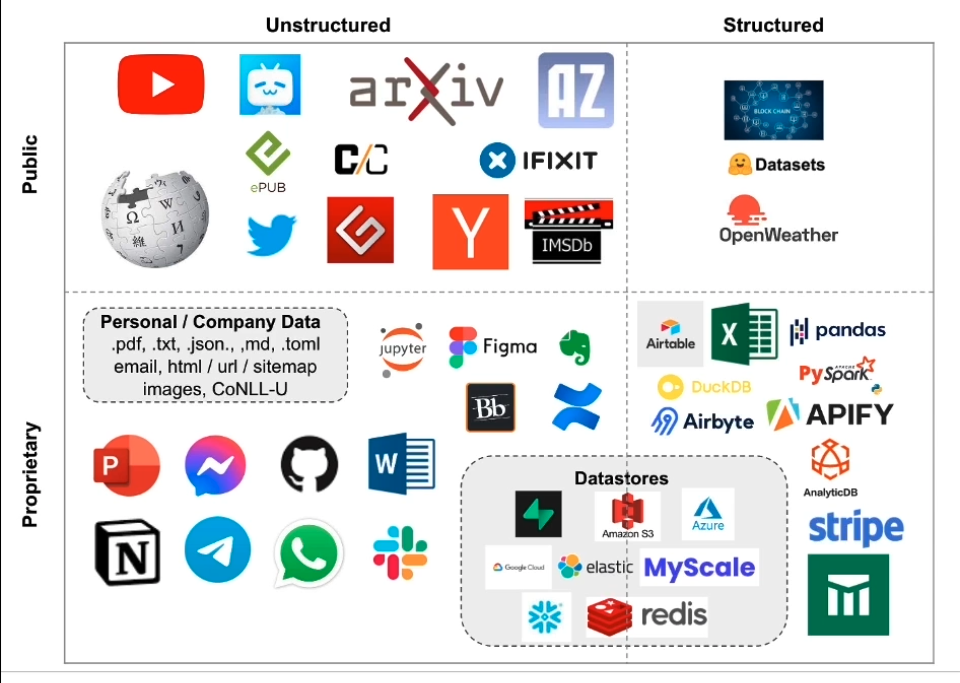
\includegraphics[width=0.8\textwidth]{images/langchain_chat_with_your_data_003.png}
    \caption{Document Loading - Types of Document Loaders}
    \label{fig:document_loading_types_of_document_loaders}
\end{figure}

%%%%%%%%%%%%%% SUBSUBSECTION %%%%%%%%%%%%%%
\subsubsection{Loading Unstructured Data}
Many document loaders deal with unstructured data, such as:
\begin{itemize}
    \item Text files
    \item Public data sources like YouTube, Twitter, and Hacker News
    \item Proprietary data sources like Figma and Notion
\end{itemize}

%%%%%%%%%%%%%% SUBSUBSECTION %%%%%%%%%%%%%%
\subsubsection{Loading Structured Data}
Some document loaders are designed for structured data, such as tabular formats. These can be useful for question-answering and semantic search applications. Sources include:
\begin{itemize}
    \item Airbyte
    \item Stripe
    \item Airtable
\end{itemize}

%%%%%%%%%%%%%%%%% SUBSECTION %%%%%%%%%%%%%%%%%
\subsection{Using Document Loaders in Practice}

See code.

%%%%%%%%%%%%%% SUBSUBSECTION %%%%%%%%%%%%%%
\subsubsection{Loading PDFs with PyPDF}
The first type of document we will work with is PDFs. To do this, we will:
\begin{itemize}
    \item Import the relevant document loader from LangChain.
    \item Use the PyPDF loader.
    \item Select a PDF from the documents folder in the workspace.
    \item Load the documents by calling the \texttt{load()} method.
\end{itemize}

By default, the loader will return a list of documents. For example, if a PDF has 22 pages, each page will be treated as a separate document. 

Each document consists of:
\begin{itemize}
    \item \textbf{Page content}: the textual content of the page.
    \item \textbf{Metadata}: information such as the file name and the page number it was loaded from.
\end{itemize}

%%%%%%%%%%%%%% SUBSUBSECTION %%%%%%%%%%%%%%
\subsubsection{Loading YouTube Transcripts}

YouTube videos contain a wealth of information, and many users want to extract transcripts for further analysis. To load YouTube transcripts, we:

\begin{itemize}
    \item Import the YouTube audio loader.
    \item Use the OpenAI Whisper parser, a speech-to-text model, to convert the audio into text.
    \item Specify a YouTube URL and a directory to save audio files.
    \item Call the \texttt{load()} function to extract the transcript.
\end{itemize}

Once completed, we can analyze the transcript and use it for further processing.

%%%%%%%%%%%%%% SUBSUBSECTION %%%%%%%%%%%%%%
\subsubsection{Loading Web Pages - URL}

The next set of documents that we're going to go over how to load are URLs from the Internet. There is a vast amount of educational content available on the internet. Wouldn't it be great if you could chat with it? We can enable this by:

\begin{itemize}
    \item Importing the \texttt{WebBaseLoader} loader from LangChain.
    \item Choosing a URL (e.g., a markdown file from GitHub).
    \item Creating a loader for the chosen URL.
    \item Calling the \texttt{load()} function to retrieve the content.
\end{itemize}

Since web pages often contain extraneous white spaces or formatting issues, some post-processing may be required to clean the data.

%%%%%%%%%%%%%% SUBSUBSECTION %%%%%%%%%%%%%%
\subsubsection{Loading Notion Data}

Notion is a popular tool for personal and company-wide knowledge management. Many people have created chatbots that interact with their Notion databases. 

To load Notion data:

\begin{itemize}
    \item Export the Notion database into a compatible format (see notebook for details).
    \item Use the Notion directory loader to load the exported data (\texttt{NotionDirectoryLoader}).
    \item Convert the data into a standard document format.
\end{itemize}

Since Notion data is often in markdown format, some users may need to preprocess the text to suit their use case.

%%%%%%%%%%%%%%%%% SUBSECTION %%%%%%%%%%%%%%%%%
\subsection{The Next Steps: Splitting Documents}

Now that we’ve covered how to load data from different sources, the next step is breaking down these documents into smaller chunks.

\begin{figure}[H]
    \centering
    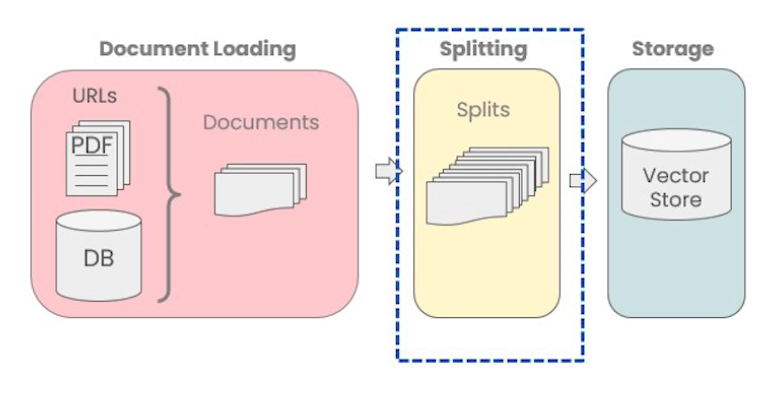
\includegraphics[width=0.8\textwidth]{images/langchain_chat_with_your_data_004.png}
    \caption{Document Loading - Next Steps}
    \label{fig:document_loading_next_steps}
\end{figure}

This is crucial for retrieval-augmented generation (RAG) applications, where we only want to retrieve the most relevant pieces of content rather than entire documents.

When retrieving information, it is inefficient to process an entire document. Instead, we should focus only on the relevant sections. This involves:

\begin{itemize}
    \item Extracting only the most topical paragraphs or sentences.
    \item Ensuring efficient retrieval by structuring content into smaller chunks.
\end{itemize}

%%%%%%%%%%%%%%%%% SUBSECTION %%%%%%%%%%%%%%%%%
\subsection{Conclusion}

We've explored how to load documents from a variety of sources and standardize them into a common document interface. However, since documents can be large, the next logical step is learning how to split them into manageable sections.

%%%%%%%%%%%%%%%%%%%% SECTION %%%%%%%%%%%%%%%%%%%%
\section{Document Splitting}

We just went over how to load documents into a standard format. Now, we’re going to talk about how to split them into smaller chunks. This may sound simple, but there are many subtleties that make a big impact down the line.

\subsection{The Importance of Document Splitting}

Document splitting happens after you load your data into the document format but before it goes into the vector store. While it may seem straightforward to split chunks based on character length, this approach can lead to issues.

\begin{figure}[H]
    \centering
    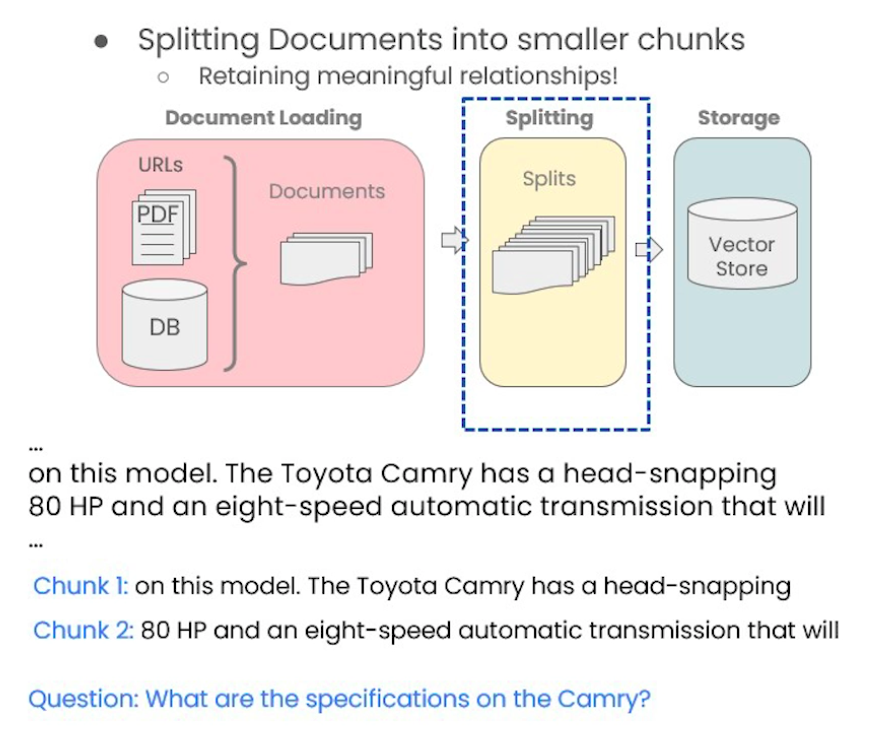
\includegraphics[width=0.6\textwidth]{images/langchain_chat_with_your_data_005.png}
    \caption{The Importance of Document Splitting}
    \label{fig:the_importance_of_document_splitting}
\end{figure}

For example, consider a sentence about the Toyota Camry and its specifications. If we simply split the text into equal parts, one chunk may contain half of the information while the other chunk holds the rest. This fragmentation can lead to incomplete responses when answering questions about the Camry’s specifications.

To prevent loss of important information, chunks should be split in a way that ensures semantically relevant text remains together.

\subsection{Text Splitters in LangChain}

LangChain provides text splitters that allow control over:

\begin{itemize}
    \item \textbf{Chunk Size}: Defines the size of each chunk.
    \item \textbf{Chunk Overlap}: Ensures that consecutive chunks contain some overlapping content to maintain context (like a sliding window).
\end{itemize}

\begin{figure}[H]
    \centering
    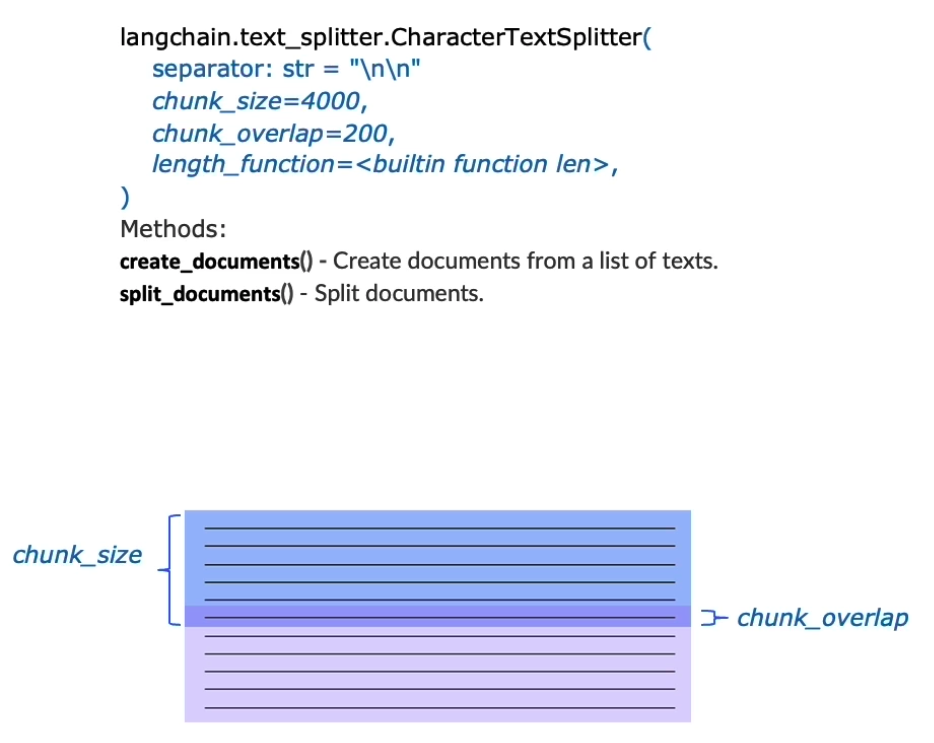
\includegraphics[width=0.6\textwidth]{images/langchain_chat_with_your_data_006.png}
    \caption{Text Splitters in LangChain - Example Splitter}
    \label{fig:text_splitters_in_langchain_example_splitter}
\end{figure}

A visual representation of chunking shows how the same piece of context can appear at the end of one chunk and at the start of the next, ensuring consistency.

A common approach involves using chunk overlap as a sliding window, ensuring that overlapping content appears at the end of one chunk and the beginning of the next.

The size of a chunk can be measured in different ways:
\begin{itemize}
    \item Number of characters
    \item Number of tokens
\end{itemize}

LangChain allows for passing a length function to define how chunk size is measured.

The Text Splitters in LangChain all have a:
\begin{itemize}
    \item create\_documents(): create documents from a list of texts.
    \item split\_documents(): split documents.
\end{itemize}

\subsection{Types of Splitters}

LangChain includes multiple text splitters with different methods of chunking. The \texttt{RecursiveCharacterTextSplitter} and the \texttt{CharacterTextSplitter} are two commonly used approaches.

\begin{figure}[H]
    \centering
    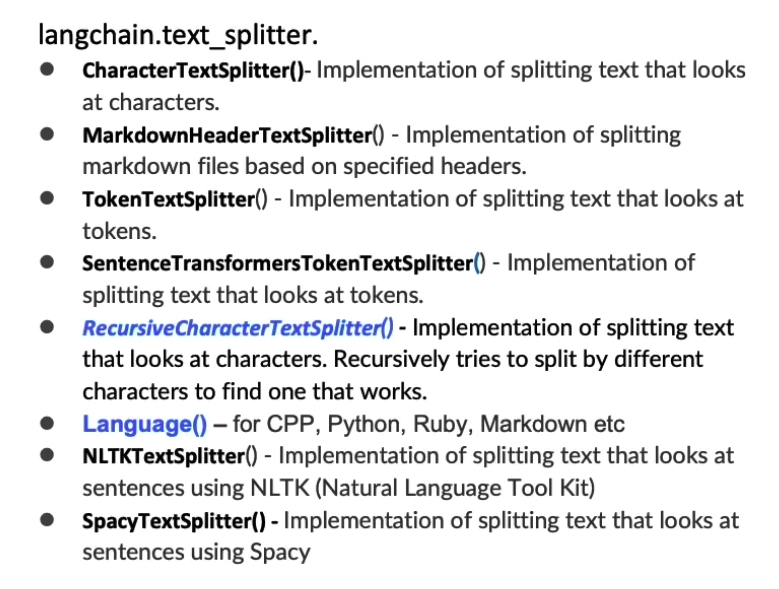
\includegraphics[width=0.5\textwidth]{images/langchain_chat_with_your_data_007.png}
    \caption{Text Splitters in LangChain - Types of Splitters}
    \label{fig:text_splitters_in_langchain_types_of_splitters}
\end{figure}

Text splitters can differ in:

\begin{itemize}
    \item How they split text (e.g., characters, sentences, paragraphs).
    \item How they measure chunk length (characters, tokens).
    \item Whether they use AI models to determine logical breakpoints.
\end{itemize}

\subsection{Maintaining Metadata}

When splitting text, it is important to retain metadata such as:

\begin{itemize}
    \item Source of the document
    \item Page number
    \item Relative position within the document
\end{itemize}

This metadata ensures that additional context is available when retrieving information.

Maintaining metadata across chunks is important, but sometimes new metadata should be added to capture the chunk’s position or relevance.

\subsection{Code-Specific Splitters}

LangChain provides splitters designed for programming languages like Python, Ruby, and C. These account for logical separators in code.

\subsection{Code Example}

See code.

\subsection{Conclusion}
We have explored various text splitting methods in LangChain, including character-based, token-based, and markdown-based techniques. We also discussed the importance of chunk overlap, metadata retention, and logical splitting for semantic relevance.

The next step is moving these processed chunks into a vector store, which we will cover in the following section.

%%%%%%%%%%%%%%%%%%%% SECTION %%%%%%%%%%%%%%%%%%%%
\section{Vector Stores and Embedding}

We've now got our document split up into small, semantically meaningful chunks, and it's time to put these chunks into an index so that we can easily retrieve them when answering questions about the corpus of data. 

To accomplish this, we will utilize \textbf{embeddings} and \textbf{vector stores}. These are critical components for building chatbots that can understand and retrieve data efficiently.

\begin{figure}[H]
    \centering
    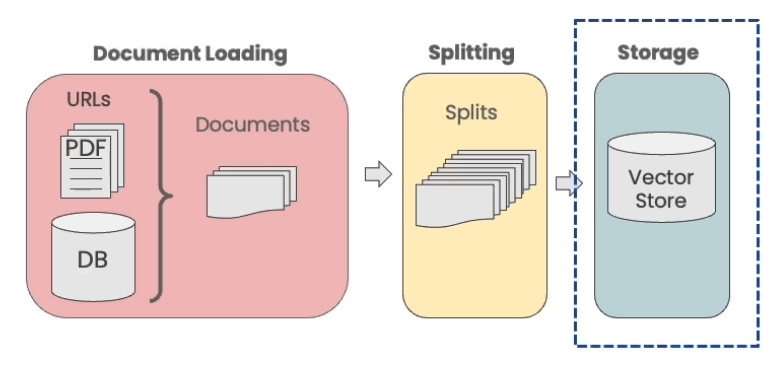
\includegraphics[width=0.6\textwidth]{images/langchain_chat_with_your_data_008.png}
    \caption{Vector Stores - Schema}
    \label{fig:vector_stores_schema}
\end{figure}

\subsection{Understanding Embeddings}

Embeddings take a piece of text and create a numerical representation of that text. Text with similar content will have similar vectors in the numeric space. This allows us to compare vectors and find similar pieces of text efficiently.

Consider the following:

\begin{figure}[H]
    \centering
    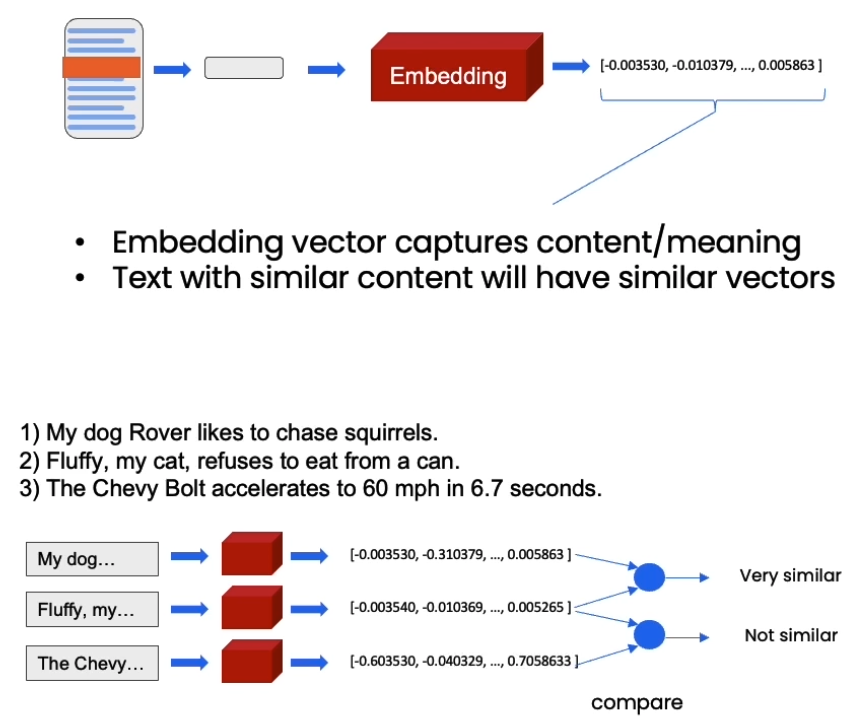
\includegraphics[width=0.7\textwidth]{images/langchain_chat_with_your_data_009.png}
    \caption{Understanding Embeddings}
    \label{fig:understanding_embeddings}
\end{figure}

\begin{itemize}
    \item Two sentences about pets will have similar vector representations.
    \item A sentence about a pet and a sentence about a car will not be similar.
\end{itemize}

\subsection{End-to-End Workflow}

The full workflow involves:

\begin{enumerate}
    \item \textbf{Starting with documents.}
    \item \textbf{Splitting them into smaller chunks.}
    \item \textbf{Creating embeddings for each chunk.}
    \item \textbf{Storing embeddings in a vector store.}
\end{enumerate}

\subsection{Using Vector Stores}

A \textbf{vector store} acts as a database that enables fast lookup of similar vectors when retrieving relevant information.

This is useful when we want to retrieve relevant documents from a question at hand. We can:

\begin{figure}[H]
    \centering
    \begin{minipage}{0.49\textwidth}
        \centering
        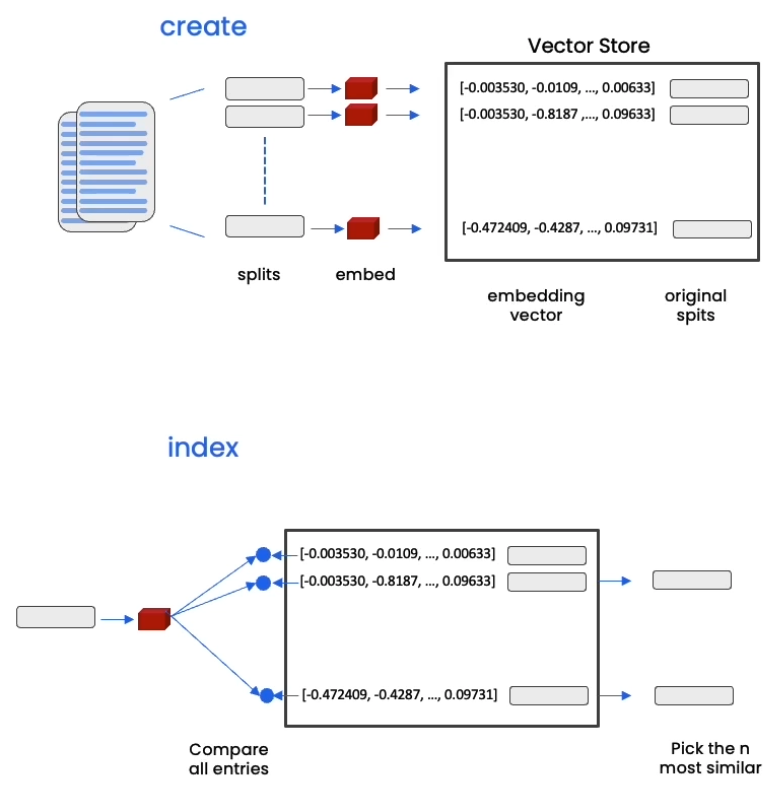
\includegraphics[width=\textwidth]{images/langchain_chat_with_your_data_010.png}
        \caption{Using Vector Stores}
        \label{fig:using_vector_stores}
    \end{minipage}
    \hfill
    \begin{minipage}{0.49\textwidth}
        \centering
        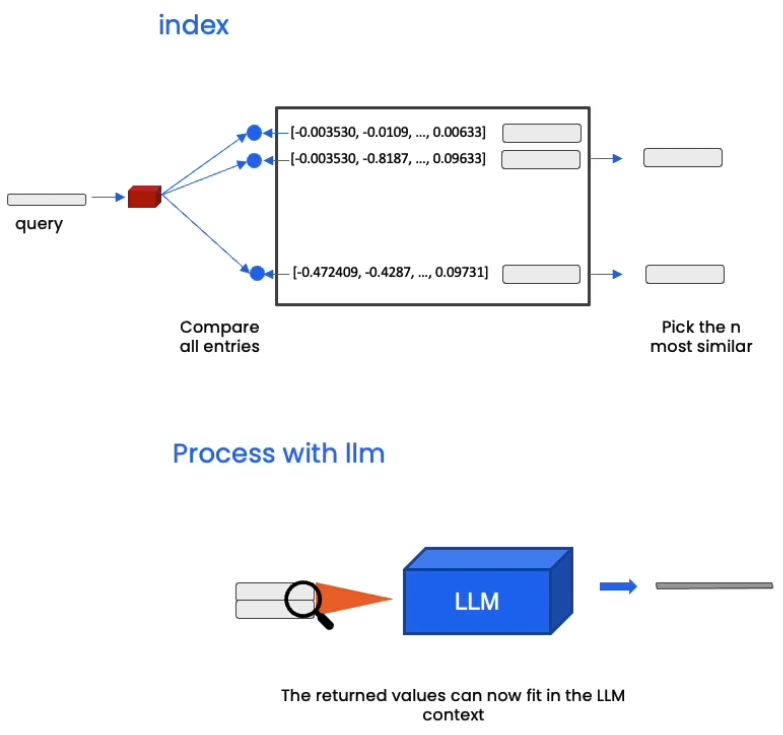
\includegraphics[width=\textwidth]{images/langchain_chat_with_your_data_011.png}
        \caption{Using Vector Stores}
        \label{fig:using_vector_stores_2}
    \end{minipage}
\end{figure}


\begin{enumerate}
    \item Convert the user’s query into an embedding.
    \item Compare this embedding against stored vectors in the vector store.
    \item Retrieve the top \texttt{n} most similar chunks.
    \item Pass the retrieved chunks along with the query to an LLM.
    \item Obtain a relevant response.
\end{enumerate}

\subsection{Code Example}

See code.

The code covers the basics about semantic search, but it isn't perfect. We will go over some edge cases and show where it can fail:

\begin{itemize}
    \item Duplicate entries: we will have the same information in two different chunks. And we will pass the same information twice to the LLM.
    \item We will ask a question related to a specific document, but the retrieval process returns information from multiple documents instead of just the intended one:

% Note section
\begin{tcolorbox}[colback=gray!10, colframe=white, width=\textwidth, sharp corners=south]
\begin{center}
\textit{What did they say about regression in the third lecture?}
\end{center}
Expected behavior: All retrieved documents should be from \textbf{Lecture 3}. 

However, results include documents from: Lecture 1, 2 and 3.

This fails because:

\begin{itemize}
    \item The phrase \textit{third lecture} is a piece of structured information.
    \item The vector search focuses primarily on the \textit{regression} term rather than lecture-specific metadata.
\end{itemize}

For example, the retrieved chunk from Lecture 1 does mention \textit{regression}, but it does not belong to Lecture 3.
\end{tcolorbox}

While the metadata contains structured details about each document, our current approach relies solely on semantic similarity, disregarding the structured metadata.
\end{itemize}

%%%%%%%%%%%%%%%%%%%% SECTION %%%%%%%%%%%%%%%%%%%%
\section{Retrieval}

In the last lesson, we covered the basics of semantic search and saw that it worked well for many use cases. However, we also encountered some edge cases where retrieval could fail. In this lesson, we will explore advanced retrieval techniques to overcome these challenges and improve search accuracy.

\subsection{Retrieval in Semantic Search}

Retrieval is crucial at query time, ensuring that we fetch the most relevant document chunks based on a given query.

\begin{figure}[H]
    \centering
    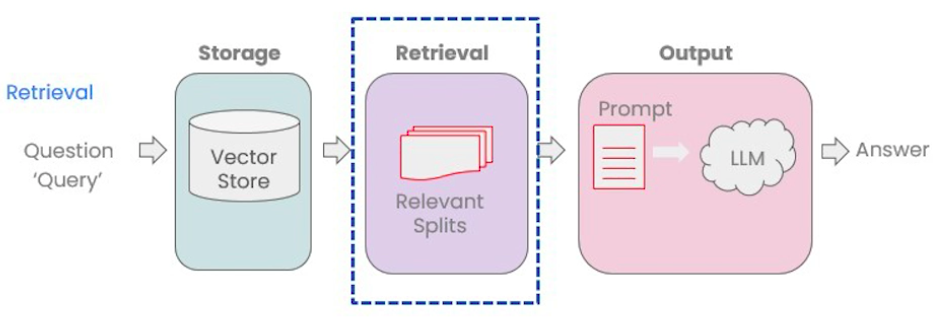
\includegraphics[width=0.8\textwidth]{images/langchain_chat_with_your_data_012.png}
    \caption{Understanding Embeddings}
    \label{fig:understanding_embeddings}
\end{figure}

Previously, we discussed semantic similarity search. Now, we will introduce more advanced retrieval methods:

\begin{enumerate}
    \item Maximum Marginal Relevance (MMR)
    \item Self-Query Retrieval
    \item Contextual Compression
    \item Alternative Retrieval Strategies (SVM, TF-IDF)
\end{enumerate}

\subsection{Maximum Marginal Relevance (MMR)}

The primary issue with basic similarity search is that it may return redundant results instead of providing diverse information.

Consider a chef asking about white mushrooms:

\begin{figure}[H]
    \centering
    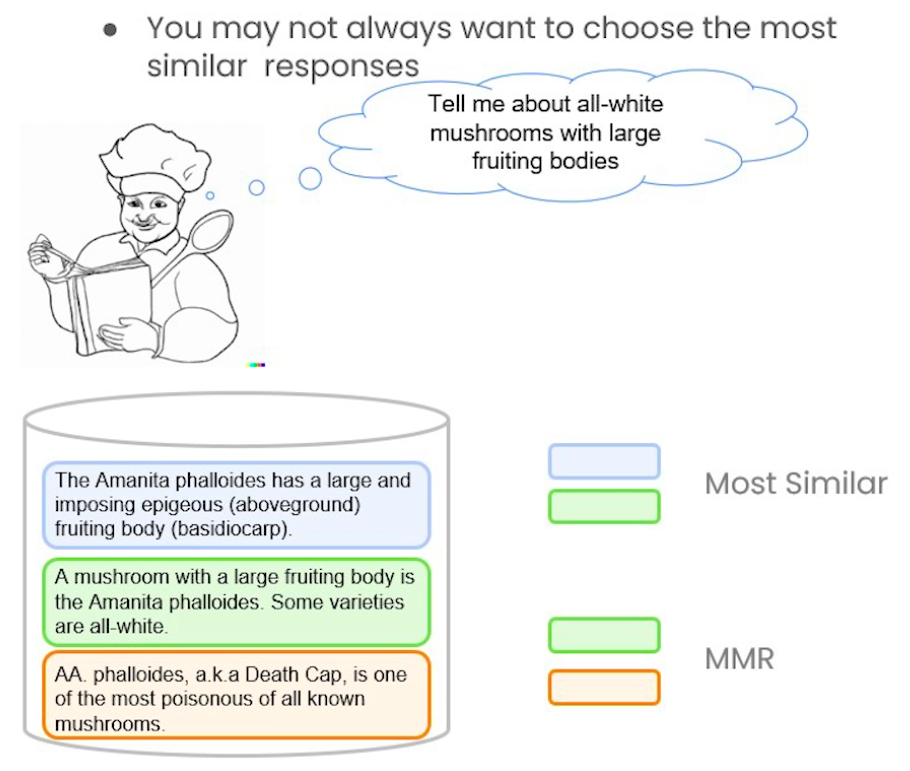
\includegraphics[width=0.5\textwidth]{images/langchain_chat_with_your_data_013.png}
    \caption{Maximum Marginal Relevance (MMR)}
    \label{fig:maximum_marginal_relevance_mmr}
\end{figure}

\begin{itemize}
    \item The most similar results might focus on the mushroom’s appearance.
    \item However, critical information like its toxicity could be missing.
\end{itemize}

\subsubsection{How MMR Works}

The idea behind MMR is that we send a query in, and then initially get back a set of responses, with \texttt{fetch\_k} being a parameter that we can control in order to determine how many responses we get. This is based solely on semantic similarity. From there, we then work with that smaller set of documents and optimize for not only the most relevant ones, based on semantic similarity, but also ones that are diverse. And from that set of documents, we choose a final "k" to return to the user.

\begin{figure}[H]
    \centering
    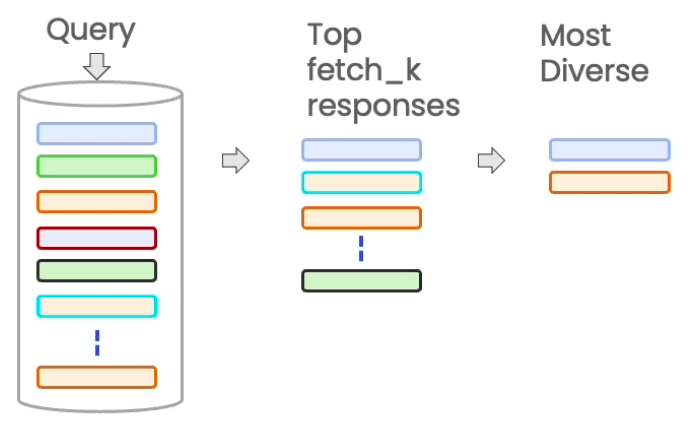
\includegraphics[width=0.5\textwidth]{images/langchain_chat_with_your_data_014.png}
    \caption{MMR - Algorithm}
    \label{fig:mmr_algorithm}
\end{figure}

\begin{enumerate}
    \item Initially retrieving a large number (\texttt{fetch\_k}) of relevant results.
    \item Selecting results that are both relevant and diverse.
    \item Returning the final \texttt{k} documents to the user.
\end{enumerate}

\subsection{LLM Aided Retrieval}

Another type of retrieval we can do is what we call \textbf{self-query}. So this is useful when you get questions that aren't solely about the content that you want to look up semantically, but also include some mention of some metadata that you want to do a filter on. Some queries contain structured metadata information alongside semantic content.

Consider the query: "What are some movies about aliens made in 1980?"

\begin{figure}[H]
    \centering
    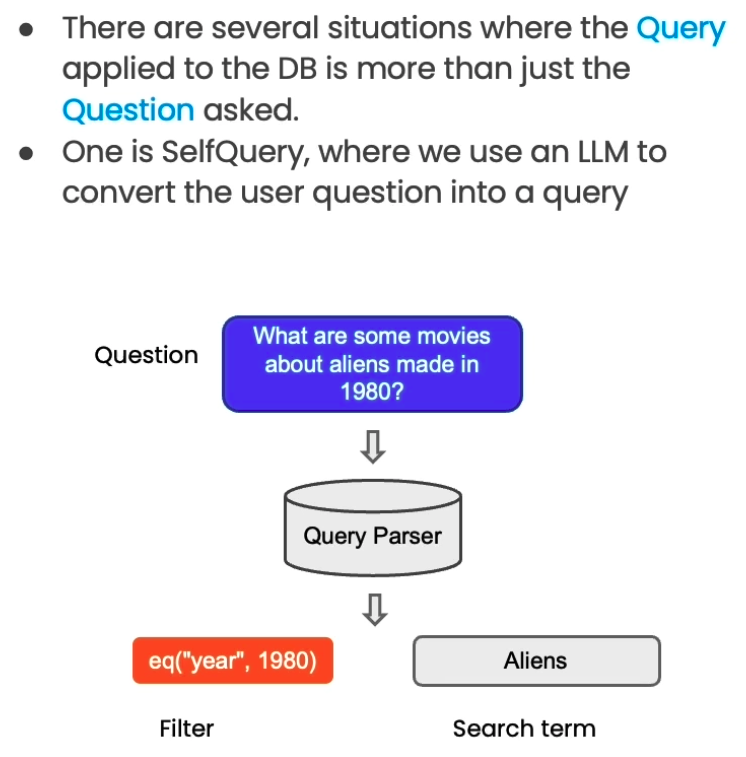
\includegraphics[width=0.4\textwidth]{images/langchain_chat_with_your_data_015.png}
    \caption{Self-Query}
    \label{fig:self_query}
\end{figure}

This really has two components to it:

\begin{itemize}
    \item \textbf{Semantic part}: Find movies about aliens.
    \item \textbf{Metadata part}: Filter results by the year 1980.
\end{itemize}

We can use a language model itself to split that original question into two separate things, a filter and a search term. Most vector stores support a metadata filter. So we can filter records based on metadata like the yea being 1980. 

\begin{itemize}
    \item Split the query into search terms and filters.
    \item Apply a metadata filter to retrieve only the relevant results.
\end{itemize}

\subsection{Compression}

This can be useful to really pull out only the most relevant bits of the retrieved passages.

\begin{figure}[H]
    \centering
    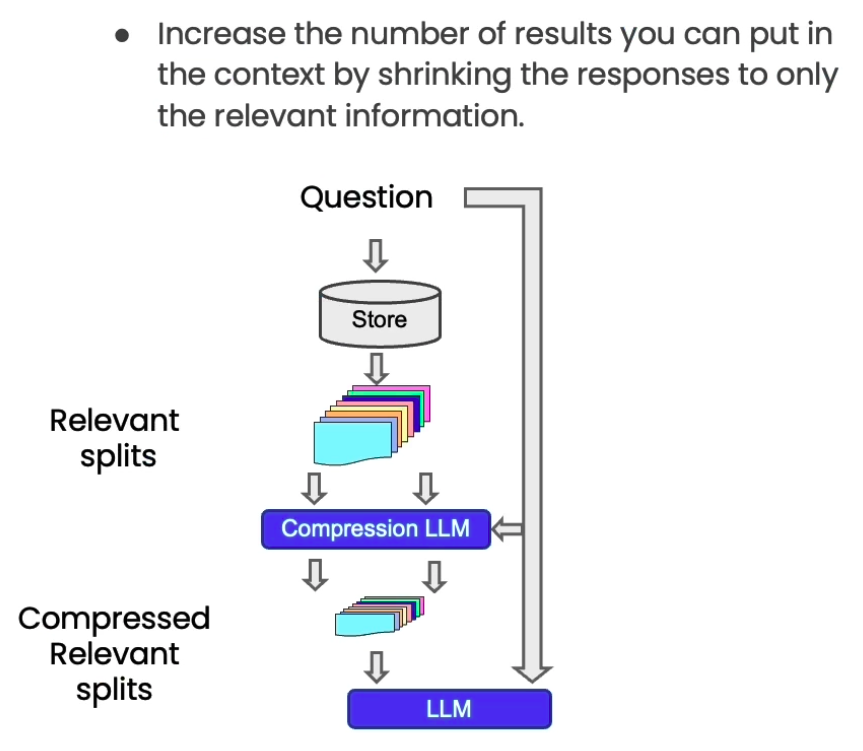
\includegraphics[width=0.5\textwidth]{images/langchain_chat_with_your_data_016.png}
    \caption{Compression}
    \label{fig:compression}
\end{figure}

For example, when asking a question, you get back the whole document that was stored, even if only the first one or two sentences are the relevant parts. With compression, you can then run all those documents through a language model and extract the most relevant segments and then pass only the most relevant segments into a final language model call.

This comes at the cost of making more calls to the language model, but it's also really good for focusing the final answer on only the most important things. And so it's a bit of a tradeoff.

\begin{enumerate}
    \item Retrieve full documents, even if only a few sentences are relevant.
    \item Run them through an LLM-based compressor (extracts only the most relevant information).
    \item Keep only the essential segments.
\end{enumerate}

\textbf{Trade-offs:}

\begin{itemize}
    \item Improves answer relevance.
    \item Requires additional LLM calls (increased computational cost).
\end{itemize}

\subsection{Alternative Retrieval Methods}

Beyond vector search, there are alternative retrieval strategies:

\subsubsection{Traditional NLP-Based Retrieval}

Some methods do not rely on vector databases:
\begin{itemize}
    \item TF-IDF retrieval
    \item Support Vector Machines (SVM) retrieval
\end{itemize}

\section{Conclusion}
This lesson introduced advanced retrieval techniques that improve search performance:
\begin{itemize}
    \item MMR for diversity.
    \item Self-query retrieval for metadata filtering.
    \item Contextual compression for focused responses.
\end{itemize}

The SelfQuery retriever in particular is my favorite, so I would suggest trying that out with more and more complex metadata filters. Even maybe making up some metadata where there's really nested metadata structures and you can try to get the LLM to infer that.

Now that we've covered retrieval techniques, the next step is to use these retrieved documents to answer user questions effectively.

%%%%%%%%%%%%%%%%%%%% SECTION %%%%%%%%%%%%%%%%%%%%
\section{Question Answering}

We've gone over how to retrieve documents that are relevant for a given question. The next step is to take those documents, take the original question, pass them both to a language model, and ask it to answer the question. We will go over that in this lesson and explore different ways to accomplish this task.

\subsection{Overview of the Process}

We will cover how to perform question answering with the documents that have just been retrieved. This follows the storage and ingestion steps, where we retrieve relevant document splits and pass them to a language model to obtain an answer.

\begin{figure}[H]
    \centering
    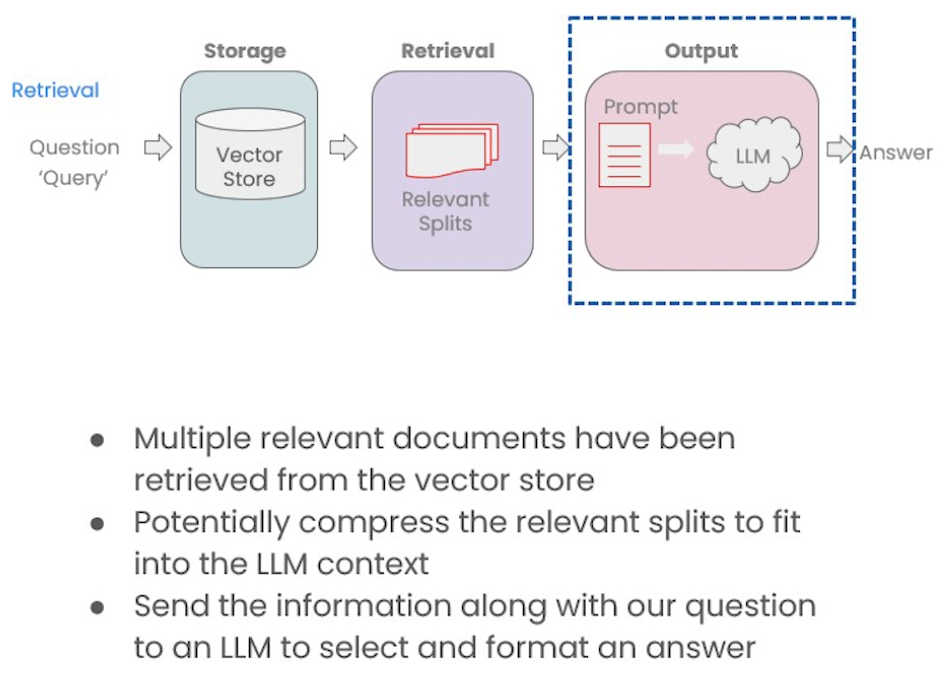
\includegraphics[width=0.7\textwidth]{images/langchain_chat_with_your_data_017.png}
    \caption{Question Answering - Schema}
    \label{fig:question_answering_schema}
\end{figure}

The general process is as follows:

\begin{figure}[H]
    \centering
    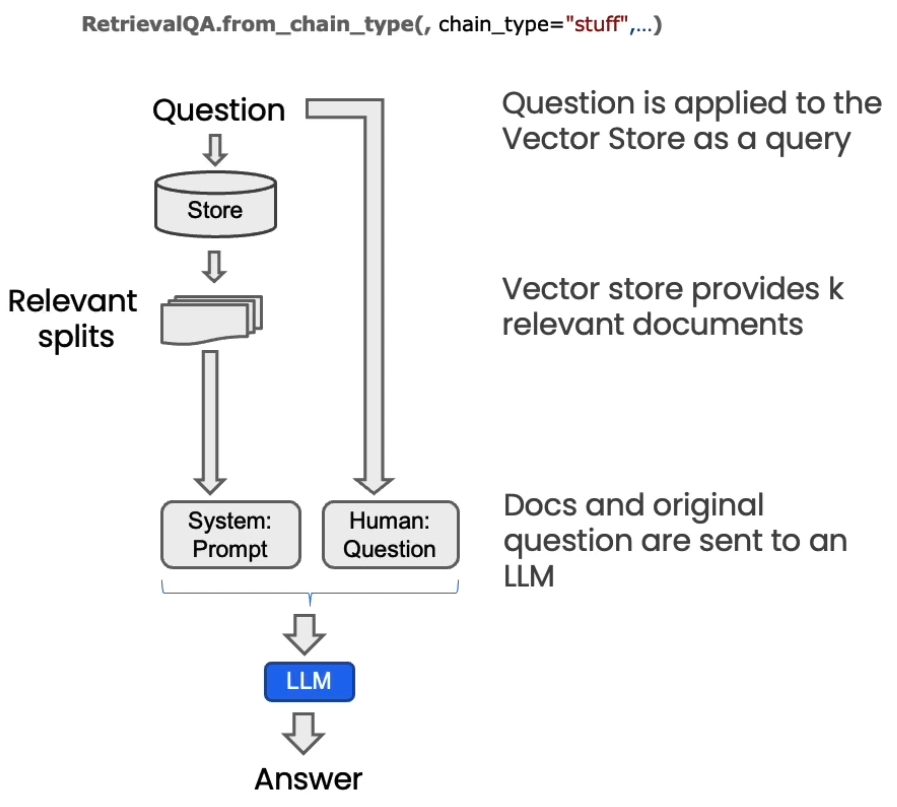
\includegraphics[width=0.7\textwidth]{images/langchain_chat_with_your_data_018.png}
    \caption{RetrievalQA Chain}
    \label{fig:retrievalqa_chain}
\end{figure}

\begin{itemize}
    \item A question is inputted.
    \item Relevant documents are retrieved.
    \item The splits of the retrieved documents, along with a system prompt and the human question, are passed to the language model.
    \item The model generates an answer.
\end{itemize}

\subsection{Handling Context Windows}

By default, all retrieved chunks are passed into the same context window during the language model call. However, there are few different methods we can use that have pros and cons to that. Most of the pros come from the fact that sometimes there can be a lot of documents and you just can't simply pass them all into the same context window.

However, there are alternative methods that address potential limitations:

\begin{itemize}
    \item \textbf{MapReduce} - Each document is processed individually, and answers are aggregated.
    \item \textbf{Refine} - The answer is iteratively refined using additional context.
    \item \textbf{MapRerank} - Answers are ranked based on relevance.
\end{itemize}

These methods help manage scenarios where too many documents exist to fit into a single context window.

\begin{figure}[H]
    \centering
    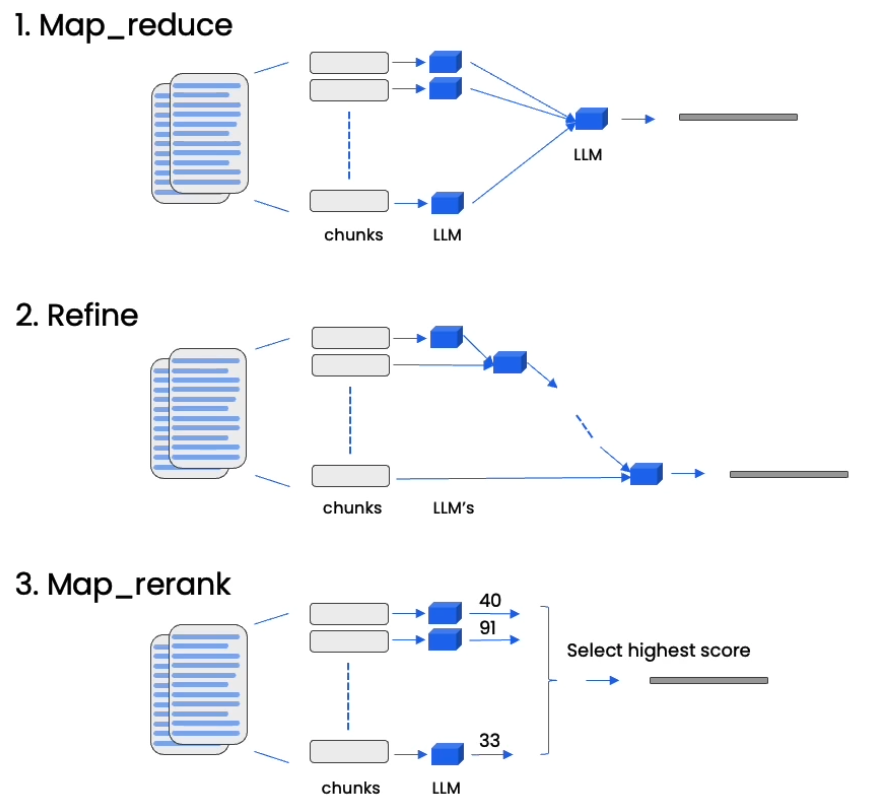
\includegraphics[width=0.7\textwidth]{images/langchain_chat_with_your_data_019.png}
    \caption{Handling Context Windows - Alternative methods}
    \label{fig:handling_context_windows_alternative_methods}
\end{figure}

\subsection{Code Example}

See code.

\subsubsection{Exploring Different QA Techniques}

\paragraph{Stuffing Technique} 
The simplest method involves stuffing all retrieved documents into a single prompt. This is efficient since it only requires one language model call, but it is limited by the context window size.

\paragraph{MapReduce Technique} 
This method first processes each document individually before aggregating the results. While it allows handling of more documents, it introduces latency and can lead to fragmented responses if the answer is spread across multiple documents.

\paragraph{Refine Technique} 
In this approach, an initial response is generated and then sequentially refined with additional context from retrieved documents. This method tends to yield more complete answers compared to MapReduce.

\subsubsection{Map Reduce Limitations}
When we use Map Reduce technique, each of the individual documents are first sent to the language model by itself to get an original answer. And then, those answers are composed into a final answer with a final call to the language model. This involves many more calls to the language model, but it does have the advantage in that it can operate arbitrarily many documents.

When we run the previous question through this chain, we can see another limitation of this method. Or actually, we can see two:

\begin{itemize}
    \item One, it's a lot slower.
    \item Two, the result is actually worse.
\end{itemize}

There is no clear answer on this question based on the given portion of the document. This may occur because it's answering based on each document individually. And so, if there is information that's spread accross two documents, it doesn't have it all in the same context.

In the code we can see that when we use "refine" method instead of "map reduce" we will get better results. That's because using the refined chain does allow you to combine information, albeit sequentially, and it actually encourages more carrying over of information than the MapReduce chain.

\subsubsection{Analyzing the System's Behavior}

Using LangChain’s UI, we can inspect how queries are processed:
\begin{itemize}
    \item Viewing input and output for each language model call.
    \item Observing how document summaries are compiled.
    \item Understanding how refined responses improve over multiple iterations.
\end{itemize}

We also explore chatbot functionality, enabling follow-up questions for clarification. However, basic retrieval QA chains lack statefulness, meaning previous questions and answers are not remembered. To address this, memory mechanisms must be introduced, which will be covered in the next section.

%%%%%%%%%%%%%%%%%%%% SECTION %%%%%%%%%%%%%%%%%%%%
\section{Chat}

We are now close to having a fully functional chatbot. We have covered loading documents, splitting them, creating a vector store, and discussing different types of retrieval. We have also demonstrated that we can answer questions, but we still lack the ability to handle follow-up questions and maintain a real conversation. This lesson will address that challenge.

\subsection{Integrating Chat History}

To complete our chatbot, we need to introduce the concept of \textbf{chat histor}y. This refers to any previous conversations or messages exchanged with the system. By incorporating chat history, the chatbot will be able to consider past interactions when answering follow-up questions, ensuring continuity in the conversation.

\begin{figure}[H]
    \centering
    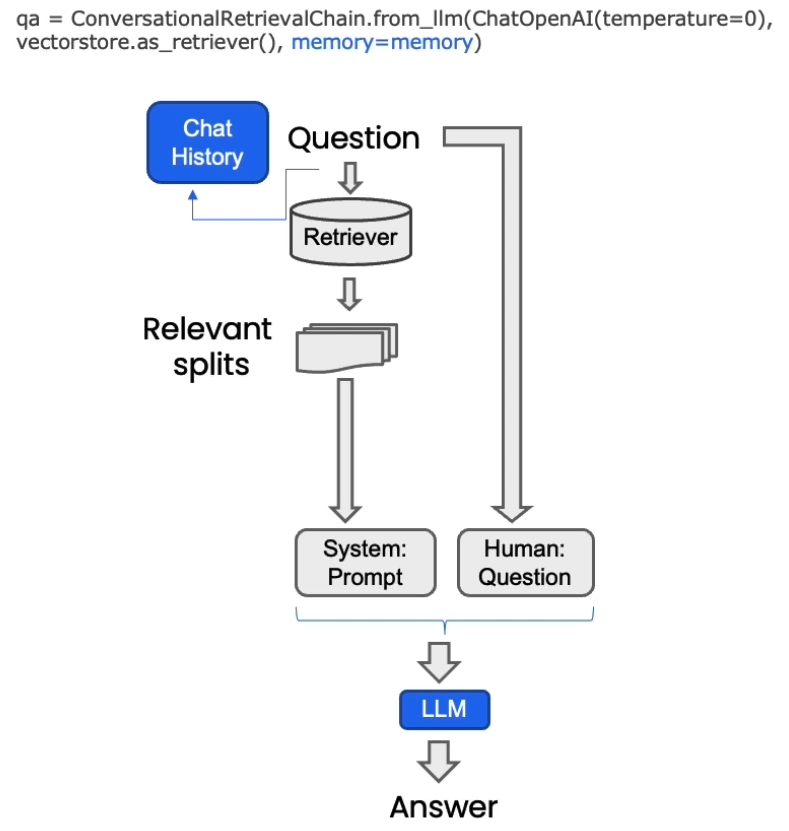
\includegraphics[width=0.5\textwidth]{images/langchain_chat_with_your_data_020.png}
    \caption{Chat - ConversationalRetrievalChain}
    \label{fig:chat_conversationalretrievalchain}
\end{figure}

An important aspect to note is that all retrieval techniques we have discussed, such as self-querying and compression, can still be applied here. The system remains modular, with chat history being an additional feature rather than a replacement of existing methods.

\begin{figure}[H]
    \centering
    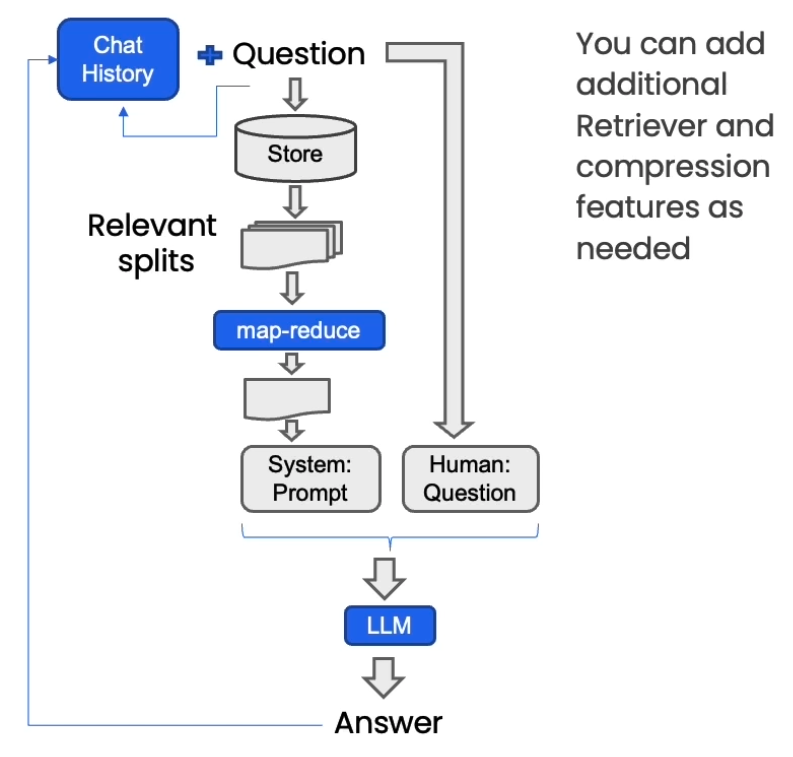
\includegraphics[width=0.6\textwidth]{images/langchain_chat_with_your_data_021.png}
    \caption{Chat - ConversationalRetrievalChain + Retrieval techniques}
    \label{fig:chat_conversationalretrievalchain_retrieval_techniques}
\end{figure}

\subsection{Code Example}

See code.

\subsubsection{Adding memory - ConversationBufferMemory}

The implementation begins by loading environment variables and initializing the vector store, which contains all the embeddings for the class materials. Next, we perform a similarity search to confirm document retrieval and initialize the language model.

Previously, we built a retrieval QA chain that could return answers to questions. Now, we extend this by adding memory to retain chat history. We use a conversation buffer memory (\texttt{ConversationBufferMemory}), which maintains a list of past chat messages and passes them along with each new question to the chatbot.

To integrate this, we specify the memory key as \texttt{chat\_history} and set \texttt{return\_messages = true}, ensuring that chat history is returned as a list of messages instead of a single string. This provides a simple and effective memory mechanism.

\subsubsection{Conversational Retrieval Chain}

We now construct a conversational retrieval chain by passing the language model, retriever, and memory as inputs. The \texttt{Conversational Retrieval Chain} adds a new bit on top of the \texttt{Retrieval QA chain}, not just memory. Specifically, what it adds is a step that takes the history and the new question and condenses it into a stand-alone question to pass to the vector store to look up relevant documents.

To test this, we ask a question without chat history and examine the result. We then ask a follow-up question and compare how the chatbot handles it. The system correctly references previous responses, improving conversational flow.

\subsubsection{Analyzing the System's Behavior}

By inspecting the system logs, we observe that the input now includes both the question and chat history. The memory module stores past interactions, ensuring context awareness. Tracing execution reveals two key steps:
\begin{itemize}
    \item A call to an LLM to reformulate follow-up questions as stand-alone queries.
    \item A call to the document retrieval module, which fetches relevant information before answering.
\end{itemize}

Examining the generated prompts, we see that the system first records previous interactions, then rephrases follow-up queries into independent questions. These reformulated questions are used to retrieve documents before generating answers.

\subsubsection{Putting It All Together}

Finally, we integrate all components into a user-friendly interface. The chatbot loads a document database, applies document chunking, generates embeddings, stores them in a vector database, and retrieves information based on user queries.

We test the chatbot by asking about the teaching assistants (TAs). The system correctly retrieves their names and can further elaborate on their backgrounds when prompted. This confirms that the chatbot retains context and supports multi-turn conversations.

\subsection{Conclusion}

This lesson has demonstrated how to build a complete question-answering chatbot using LangChain. We have covered:
\begin{itemize}
    \item Loading and chunking documents.
    \item Creating a vector store and performing semantic search.
    \item Implementing retrieval techniques and query reformulation.
    \item Introducing chat history for conversational memory.
    \item Constructing a UI for interactive chatbot interactions.
\end{itemize}

With these components, we have successfully developed an end-to-end conversational chatbot that can retrieve and process data dynamically. Future work includes experimenting with different memory mechanisms, improving query reformulation techniques, and refining retrieval algorithms. This concludes our session on LangChain-based chatbots.

\section{Conclusion of LangChain Course}

This class on LangChain, \textit{Chat with Your Data}, has come to an end. Throughout this course, we have explored how to use LangChain to load data from a variety of document sources using LangChain's extensive collection of over 80 document loaders.

\begin{figure}[H]
    \centering
    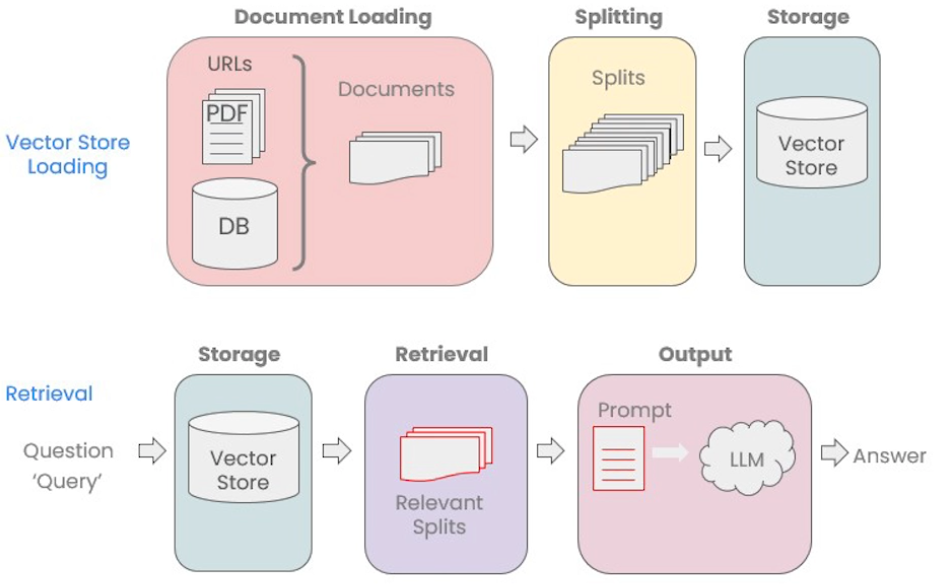
\includegraphics[width=0.8\textwidth]{images/langchain_chat_with_your_data_022.png}
    \caption{LangChain - Chat with your data}
    \label{fig:langchain_chat_with_your_data}
\end{figure}

\subsection{Key Learnings}

\subsubsection{Document Processing and Retrieval}

We learned how to:

\begin{itemize}
    \item Split documents into manageable chunks and discussed nuances that arise in this process.
    \item Create embeddings for these chunks and store them in a vector database, enabling semantic search.
    \item Understand the limitations of semantic search and the edge cases where it may fail.
\end{itemize}

\subsubsection{Retrieval Techniques}

Retrieval was one of the most engaging parts of the course, where we explored new and advanced retrieval algorithms to overcome edge cases. We then combined these techniques with large language models (LLMs) to:

\begin{itemize}
    \item Retrieve relevant document chunks based on user queries.
    \item Use an LLM to generate answers based on retrieved documents.
    \item Identify and address missing elements in traditional retrieval systems.
\end{itemize}

\subsubsection{Conversational Aspect}

The last step in our journey was building a fully functional, end-to-end chatbot that maintains context over multiple turns of conversation. This enabled the chatbot to:

\begin{itemize}
    \item Remember prior exchanges and use them to improve follow-up responses.
    \item Generate relevant answers dynamically.
    \item Provide an interactive experience for users.
\end{itemize}

\bibliographystyle{alpha}
\bibliography{sample}

\end{document}
